\section{Reflection}
Unter Reflection versteht man die Analyse von Metadaten eines Objekts zur Laufzeit. Mit Reflection lassen sich Typen suchen und instanzieren. Die abstrakte Basisklasse System.Type representiert einen Typen. System.RuntimeType erbt von System.Type. Mit Reflection können auch \lstinline{private} Felder gelesen und geschreiben werden.

\begin{figure}[h!]
	\centering
	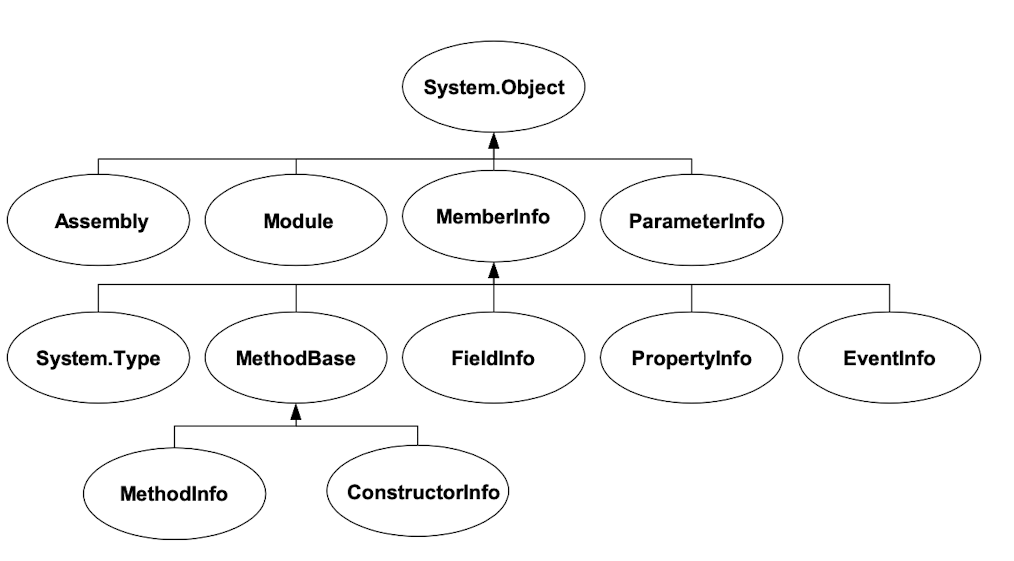
\includegraphics[width=0.8\linewidth]{typehierarchie}
	\caption{Typ-Hierarchie}
	\label{fig:valuetypes}
\end{figure}

\subsection{Anwendungen}
\begin{description}
    \item[Metadaten erstellen] Darstellung der Metadaten in Tools
    \item[Type Discovery] Suchen und Instanzieren von Typen, Zugriff auf dynamische Datenstrukturen.
    \item[Late Binding (Methods/Properties] Aufruf von Methoden / Properties nach Type Discovery
    \item[Reflection Emit / Code-Emittierung] Erstellen von Typen inkl. Members zur Laufzeit
    \item[Alle Typen in der Common Language Runtime (CLR) sind selbst-definierend]
    \item[Nicht zugreifbare Members auch einsehbar] z.b. private Felder
    \item[Klasse ''System.Type''] Einstiegspunkt aller Reflection-Operationen, repraesentiert einen Typen mit all seinen Eigenschaften, abstrakte Basisklasse, ''Sysemt.RuntimeType'' wird jeweils verwendet.
    \item[Ermitteln von ''System.Type'' via] \lstinline|"obj".GetType()|, \lstinline|typeof("classname")|.
\end{description}
\begin{lstlisting}
this.GetType() // implemented on object
typeof(MyClass) || typeof(int)
\end{lstlisting}

\subsection{Type Discovery}
Suche alle Typen in einem Assembly.
\begin{lstlisting}[caption=Reflection: Type Discovery]
Assembly a01 = Assembly.Load("mscorlib, PublicKeyToken=b77a5c561934e089, Culture=neutral, Version=4.0.0.0");
// Assembly.Load("File.dll") File auslesen
Type[] t01 = a01.GetTypes();
foreach (Type type in t01) {
	Console.WriteLine(type);
	MemberInfo[] mInfos = type.GetMembers();
	foreach (var mi in mInfos) 	{
		Console.WriteLine(
		"\t{0}\t{1}",
		mi.MemberType,
		mi);
	}
}
\end{lstlisting}


\subsection{Member auslesen}
Das Auslesen von Members kann mit \lstinline|BindingFlags| gefiltert werden.
\begin{lstlisting}[caption=Reflection: Members auslesen]
Type type = typeof(Counter);
MemberInfo[] miAll = type.GetMembers();
foreach (MemberInfo mi in miAll) {
	Console.WriteLine("{0} is a {1}", mi, mi.MemberType);
}
Console.WriteLine("----------");
PropertyInfo[] piAll = type.GetProperties();
foreach (PropertyInfo pi in piAll) {
	Console.WriteLine("{0} is a {1}",	pi, pi.PropertyType);
}

// ex2: filter members according to BindingFlag or Filtername
Type type = typeof(Assembly);
BindingFlags bf =
	BindingFlags.Public |
	BindingFlags.Static |
	BindingFlags.NonPublic |
	BindingFlags.Instance |
	BindingFlags.DeclaredOnly;

System.Reflection.MemberInfo[] miFound = type.FindMembers(
	MemberTypes.Method, bf, Type.FilterName, "Get*"
);
\end{lstlisting}

\subsection{Field Information}
Die Field Info beschreibt ein Feld einer Klasse (Name, Typ, Sichtbarkeit). Die Felder können mit \lstinline|object GetValue(object obj)| und \lstinline|void SetValue(object obj, object value)| auch gelesen und geschrieben werden.

\begin{lstlisting}[caption=Reflection: Field Info]
Type type = typeof (Counter);
Counter c = new Counter(1);

// All Fields
FieldInfo[] fiAll = type.GetFields(BindingFlags.Instance | BindingFlags.NonPublic);
	
// Specific Field
FieldInfo fi = type.GetField("countValue", BindingFlags.Instance | 	BindingFlags.NonPublic);
	
int val01 = (int) fi.GetValue(c);
c.Increment();
int val02 = (int) fi.GetValue(c);
fi.SetValue(c, -999);
\end{lstlisting}


\subsection{Property Information}
Die Property Info beschreibt eine Property einer Klasse (Name, Typ, Sichbarkeit, Informationen zu Get/Set). Auch Properties lassen sich lesen und schreiben.
\begin{lstlisting}[caption=Reflection: Property Info]
Type type = typeof(Counter);
Counter c = new Counter(1);

// All Properties
PropertyInfo[] piAll = type.GetProperties();

// Specific Property
PropertyInfo pi = type.GetProperty("CountValue");

int val01 = (int)pi.GetValue(c);
c.Increment();
int val02 = (int)pi.GetValue(c);
if(pi.canWirte) { pi.SetValue(c, -999); }
\end{lstlisting}

\subsection{Method Info}
Die Method Info beschreibt eine Methode einer Klasse (Name, Parameter, Rückgabewert, Sichtbarkeit). Sie leitet von Klasse \lstinline|MethodBase| ab. Die Methode wird mit \lstinline|Invoke()| aufgerufen.
\begin{lstlisting}[caption=Reflection: Method Info]
Type type = typeof(Counter);
Counter c = new Counter(1);

// All Methods
MethodInfo[] miAll = type.GetMethods();

// Specific Method
MethodInfo mi = type.GetMethod("Increment");
mi.Invoke(c, null);
\end{lstlisting}

\subsection{Constructor Info}
Die Constructor Info beschreibt ein Konstruktor einer Klasse (Name, Parameter, Sichtbarkeit). Wie Method Info leitet er wegen seinen ähnlichen Eigenschaften von \lstinline|MethodBase| ab und wird  mit \lstinline|Invoke()| aufgerufen.
\begin{lstlisting}[caption=Reflection: Constructor Info]
Type type = typeof(Counter);
Counter c = new Counter(1);

// All Constructors
var ciAll = type.GetConstructors();

// Specific Constructor Overload 01
ConstructorInfo ci01 = type.GetConstructor(new[] { typeof(int) });
Counter c01 = (Counter)ci01.Invoke(new object[] { 12 });

// Specific Constructor Overload 02
ConstructorInfo ci02 = type.GetConstructor(BindingFlags.Instance|BindingFlags.NonPublic, null, new Type[0], null);
Counter c02 = (Counter)ci02.Invoke(null);
\end{lstlisting}


\subsection{Example of Reflection Usage}
\begin{lstlisting}
using System.Reflection;

namespace TestReflection {
    class Program {
        static void Main(string[] args)  {
            var ass=Assembly.LoadFrom("Autos.dll");
            var t = ass.GetType("Autos.FastCars");
            var c=Activator.CreateInstance(t, new object[] {"Lamborghini"});
            var m = t.GetMethod("AutoFahren");
            m.Invoke(c, new object[]{});
        }
    }
} 
\end{lstlisting}
\pagebreak

\section{Attributes}
Attributes sind das C\# Pendant zu den Java Annotations. Bei Attributen geht es um die aspektorientierte Programmierung. z.B Erweiterung eines Attributes um eine Aspekt Serialisierung, Transactions, etc. Es können auch eigene Attribute geschrieben werden. Diese leiten immer von \lstinline|System.Attribute| ab. Attribute können mit über Reflection abgefragt werden. 
\begin{lstlisting}[caption=Attributes]
[DataContract, Serializable]
[Obsolete]
// Etc.
public class Auto {
	[DataMember]
	public string Marke { get; set; }
	[DataMember]
	public string Typ { get; set; }
}

// Beliebig viele Attribute
[DataContract][Serializabel] <=> [DataContract, Serializabel]

// Parameter
[DataContract] // Ohne Parameter
[DataContract(Name="MyParam")] // Named Parameter
[Obsolete("Alt!",  true)] // Positional Parameter
[Obsolete("Alt!", IsError=true)] // Mixed
\end{lstlisting}

\subsection{Anwendungsfälle}
\begin{itemize}
	\item Object-relationales Mapping
	\item Serialisierung (WCF, XML)
	\item Security und Zugriffsteuerung
	\item Dokumentation
\end{itemize}

\subsection{Typen}
Man unterscheidet zwei Typen von Attributen
\begin{enumerate}
	\item Intrinsic Attributes: Kommen bereits mit der CLR mit 
	\item Custom Atttributes: Eigens definierte Attributre
\end{enumerate}

\subsection{Eigene Attribute}
Bei der Deklaration können die Objekte eingegrenzt werden, auf die das Attribute angewendet werden kann. Jedes Attribute muss als Postfix ''Attribute'' haben. (xxAttribute). Beim Verwenden wird der Postfix jedoch weggelassen.
\begin{lstlisting}
// declaration 
[AttributeUsage(                    //definiert wo attribute verwendet werden duerfen
	AttributeTargets.Class |
	AttributeTargets.Constructor |
	AttributeTargets.Field |
	AttributeTargets.Method |
	AttributeTargets.Property,
	AllowMultiple = true)]
public class BugfixAttribute : Attribute
{
	public BugfixAttribute(int bugId, string programmer, string date) {..}
	public int BugId { get; }
	public string Date { get; }
	public string Programmer { get; }
	public string Comment { get; set; }
}

// usage
[Bugfix(121, "MichaelWieland", "14/12/16")]
\end{lstlisting}
\textbf{CSV-Filter}
\begin{lstlisting}
// list
var a = new List<Address> {
	new Address("Hans", "Strasse 16", "8645", "Jona") ,
	new Address("Hans2", "Strasse 2", "8645", "Jona")
}
Writer.SaveToCsv(a, @"C:\Temp\test.csv");

// address
public class Address {
	[CsvName("Name"), Uppercase]
	public string Name { get; set; }
	[CsvName("Strasse"), Lowercase]
	public string Street { get; set; }
	[CsvName("Plz")]
	public string Postcode { get; set; }
	...
}

// Custom Attributes
public class CsvNameAttribute : Attribute {     // Mapping eines Properties auf CSV Spalte
	public string Name { get; set; }
	public CsvAttribute(string name) {
		Name = name;
	}
}

public interface IStringFilter {            // beschreibt beliebigen Filter
	string Filter(string arg); 
}
public class UppercaseAttribute : Attribute : IStringFilter {       // Implementation von IStringFilter
	public string Filter(string arg) {
		return arg.ToUpper();
	}
}
public class LowercaseAttribute : Attribute : IStringFilter {       // Implementation von IStringFilter
	public string Filter(string arg) {
		return arg.ToLower();
	}
}
\end{lstlisting}

\subsection{Reflection Emit}
Reflection.Emit erlaubt neue Assemblies und Typen zur Laufzeit zu erzeugen und sofort zu verwnden. Erzeugen von Assemblies, neuen Modulen, neuen Typen, symbolischer Metainformationen für bestehende Module.
\textbf{Wichtigste Klassen}
\begin{itemize}
    \item AssemblyBuilder $\Rightarrow$ Assemblies definieren
    \item ModuleBuilder $\Rightarrow$ Module definieren
    \item TypeBuilder $\Rightarrow$ Typen definieren
    \item MethodBuilder $\Rightarrow$ Methoden definieren
    \item ILGenerator $\Rightarrow$ IL-Code erzeugen
\end{itemize}

\textbf{Assembly inkl. Module definieren}
\begin{lstlisting}
AssemblyName assemblyName = new AssemblyName("Hsr.EmitDemoAssembly");
AssemblyBuilder assemblyBuilder = AppDomain.CurrentDomain.DefineDynamicAssembly(assemblyName, AssemblyBuilderAccess.RunAndSave);
ModuleBuilder moduleBuilder = assemblyBuilder.DefineDynamicModule("Hsr.EmitDemoModule", "Hsr.EmitDemoAssembly.dll");
\end{lstlisting}

\textbf{Klasse ''EmitDemo'' definieren}
\begin{lstlisting}
TypeBuilder typeBuilder = moduleBuilder.DefineType("EmitDemo", TypeAttributes.Public);
\end{lstlisting}

\textbf{Methode ''SayHello'' definieren}
\begin{lstlisting}
Type[] paramTypes = { typeof(string) };
Type retType = typeof(string);
MethodBuilder methodBuilder = typeBuilder.DefineMethod("SayHelloTo",
        MethodAttributes.Public | MethodAttributes.Virtual, retType, paramTypes);
\end{lstlisting}

\textbf{Einfügen der MSIL Operationen in die neu erzeugte Methode}
\begin{lstlisting}
ILGenerator ilGen = methodBuilder.GetILGenerator();
ilGen.Emit(OpCodes.Ldstr, "Hello ");
ilGen.Emit(OpCodes.Ldarg_1);
MethodInfo mi = typeof(string).GetMethod("Concat", new[] { typeof(string), typeof(string) });
ilGen.Emit(OpCodes.Call, mi);
ilGen.Emit(OpCodes.Ret);
\end{lstlisting}

\textbf{Klasse ''EmitDemo'' erzeugen}
\begin{lstlisting}
typeBuilder.CreateType();
\end{lstlisting}

\textbf{Methode ''SayHello'' ausführen}
\begin{lstlisting}
MethodInfo method = typeBuilder.GetMethod("SayHelloTo", new[] { typeof(string) });
object obj = Activator.CreateInstance(typeBuilder);
object ret = method.Invoke(obj, new object[] { "HSR" });
Console.WriteLine(ret);
\end{lstlisting}

\textbf{Assembly ''Hsr.EmitDemoAssembly.dll'' abspeichern}
\begin{lstlisting}
assemblyBuilder.Save(assemblyName.Name + ".dll");
\end{lstlisting}

